\documentclass[12pt]{article}

%
%Margin - 1 inch on all sides
%
\usepackage[letterpaper]{geometry}
\usepackage{times}
\geometry{top=1.0in, bottom=1.0in, left=1.0in, right=1.0in}

%
%Doublespacing
%
\usepackage{setspace}
%\doublespacing
\usepackage{hyperref}

%
%Rotating tables (e.g. sideways when too long)
%
\usepackage{rotating}
\usepackage{multicol}
\usepackage{ragged2e}

\usepackage{graphicx}
\graphicspath{{./images/}}


%
%Fancy-header package to modify header/page numbering (insert last name)
%
\usepackage{fancyhdr}
\pagestyle{fancy}
\lhead{May 8, 2023} 
\chead{\textbf{Emulating an IPS over an IDS using Iptables}} 
\rhead{John Nunley \thepage} 
\lfoot{} 
\cfoot{} 
\rfoot{} 
\renewcommand{\headrulewidth}{0pt} 
\renewcommand{\footrulewidth}{0pt} 
%To make sure we actually have header 0.5in away from top edge
%12pt is one-sixth of an inch. Subtract this from 0.5in to get headsep value
\setlength\headsep{0.333in}

%
%Works cited environment
%(to start, use \begin{workscited...}, each entry preceded by \bibent)
% - from Ryan Alcock's MLA style file
%
\newcommand{\bibent}{\noindent \hangindent 40pt}
\newenvironment{workscited}{\newpage \textbf{7). References}}{\newpage }


%
%Begin document
%
\begin{document}
\begin{flushleft}

\justifying

%%%%Changes paragraph indentation to 0.5in
\setlength{\parindent}{0.5in}
%%%%Begin body of paper here

\begin{multicols}{2}
    
\textbf{1). Abstract}

One way to turn an Intrusion Detection System (IDS) into an Intrusion Prevention System (IPS) is to connect its alerts to a firewall. The primary strategy in this case is to map alerts to new firewall rules. This paper introduces a strategy for transforming IDS alerts into firewall rules as an IPS. The strategy combines a heuristic approach where the firewall rules are only applied for a limited time with a random removal of rules. This strategy is implemented using Iptables, a Linux firewall. The results show that the strategy is effective at reducing the number of false positives and false negatives, as well as their disruption of business operations. The ultimate goal of this project is to create a tool that can be used by network administrators to turn an IDS into an IPS.

\textbf{2). Introduction}

For ensuring the continued integrity of computer networks, it is of the utmost importance to make sure no intrusions occur. Intrusions are defined as "A security event, or a combination of multiple security events, that constitutes a security incident in which an intruder gains, or attempts to gain, access to a system or system resource without having authorization to do so" (NIST, 2015). In order to ameliorate the effects of instrusions, network administrators must establish preventative controls to detect and prevent intrusion.

There are two general categories of controls. One type of system is an Intrusion Detection System (IDS), where the system analyzes incoming packets and determines if they represent an intrusion. Popular IDS systems include Snort, Bro and Security Onion (Software Testing Help, 2023). There are many different ways for an IDS to operate, like rule-bassed detection and profiling. On the other hand, there are also Intrusion Prevention Systems (IPS). The emphasis of an IPS focuses less on detection and more on stopping intrusion outright. Most packet analysis is similar to that of an IPS. Certain IDS systems, like Snort, also have an optional IPS mode (Patel et al, 2010). However, there are other IPS tools like Cisco NGIPS. The main difference between an IDS and an IPS is that an IPS can block traffic, while an IDS cannot (NIST, 2007).

At a first glance, it may seem like an IPS has an immediate advantage over an IDS. However, IPS generally have to ignore more behavior, since if they come upon a false positive, they will block valid traffic. In many cases, it's better to have logs of \textit{potentially} malicious behavior than to block valid traffic (Mohanakrishnan, 2022). 

The fact that IDS as a significant number of false positives makes it difficult to adapt an IDS as an IPS. However, with a heuristic based strategy and taking advantage of random noise, one can effectively combine an IDS with the IPTables firewall to create a rudimentary IPS.

\textbf{3). Challenges in the security issue/threat model}

The na\"{i}ve approach would be to take signatures that the underlying IDS marks as malicious and then add an entry to Iptables that blocks that IP. This approach would be easy to implement and set up. However, the problem comes in when the IDS has a false positive. A single false positive can lead to connections being interrupted, which can be very disruptive. In addition, IDS may also have true negatives, where it fails to detect malicious traffic. There are also cases where IP addresses can be spoofed, which can lead to issues when a malicious user uses a benign user's IP address (RSI Security, 2007).

The first issue must be addresses by using a heuristic based strategy. Rather than just blocking the packet signature outright, it should only be blocked for a limited time. This allows the IDS to learn from its mistakes and not block valid traffic. The time starts off at a short interval; at the moment it is around 5 minutes. Every time the IDS produes another warning with that specific signature, the time that the signature is blocked is doubled. This strategy makes sure that the IDS has time to "learn" from its mistakes, while still blocking malicious traffic.

However, given the prevalence of false positives, it is still possible for benign traffic to be blocked in this way. In order to prevent this failure, before the filter starts blocking traffic, it assigns it a "score" and ticks it down every time a flagged packet is received. For instance, when the IDS first flags a signature, it assigns it a score of five. Every time the IDS flags the same signature, the score is decremented by one. When the score reaches zero, the Iptables firewall starts filtering the packet with the above heuristic strategy. This means that innocuous clients won't be blocked, as they have a "grace period" of five warnings. However, malicious clients will be blocked for longer, as they will exhaust their grace period faster.

In order to prevent blocks from sticking for too long, the table of data above needs to "decay". This also addresses the problem of spoofed attacks; this prevents innocuous targets from being repeatedly false flagged. Randomness is introduced in order to make the table decay in this way. The filters are removed randomly, with an adjustable probability. This means that the data in the table (such as the score and the filtering duration) will start to "decay" after not being used for a while. This helps benign clients avoid being blocked for too long. The probability of a filter being removed is adjustable, so that the administrator can adjust the rate at which the table decays.

In order to test this algorithm, a na\"{i}ve visualization of a network was constructed to test this strategy. A small network of servers representing an internet is randomly generated. Most of the servers are benign; however, a few servers are set as "malicious". On the other hand, there is one other server, representing a router for a private network. This router is connected to several of the other "internet" servers. In addition, the router is connected to several "web" servers, representing web sites accessed through the larger internet.

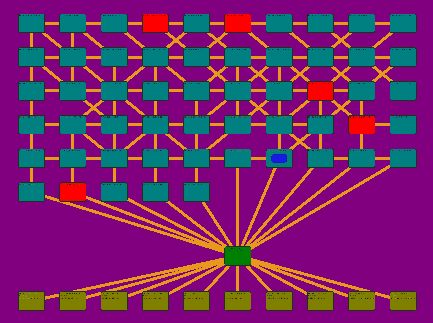
\includegraphics[scale=0.5]{cs-653-networksim.png}

Packets are sent from the internet servers to the web servers. The simulation runs on "ticks", where a packet makes a hop every tick. Benign servers produce benign packets, while malicious servers produe malicious packets. Once the packet reaches its destination, a simulation of an IDS is run on the packet. The simulation flags the packet as malicious or benign, with appoximately 33\% chance of a false positive. This information is sent to the router, where the Iptables firewall is run. If a currently filtered packet attempts to cross the router boundary, the router will drop the packet.

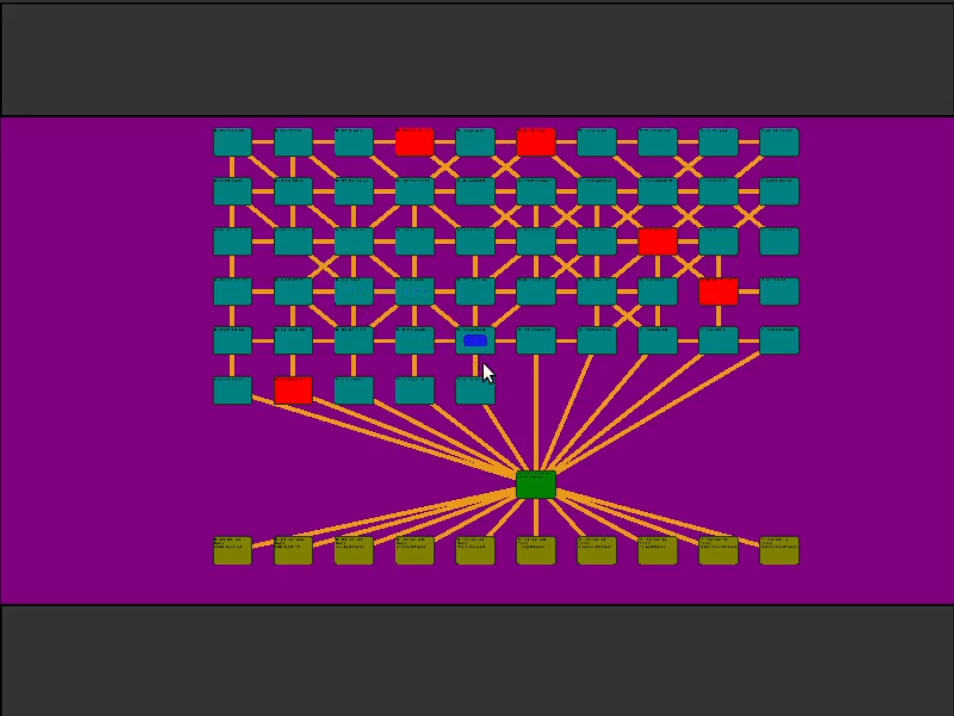
\includegraphics[scale=0.20]{screenshot2.png}

\textit{The simulation in action. Note the blue (non malicious) packet traversing network graph.}

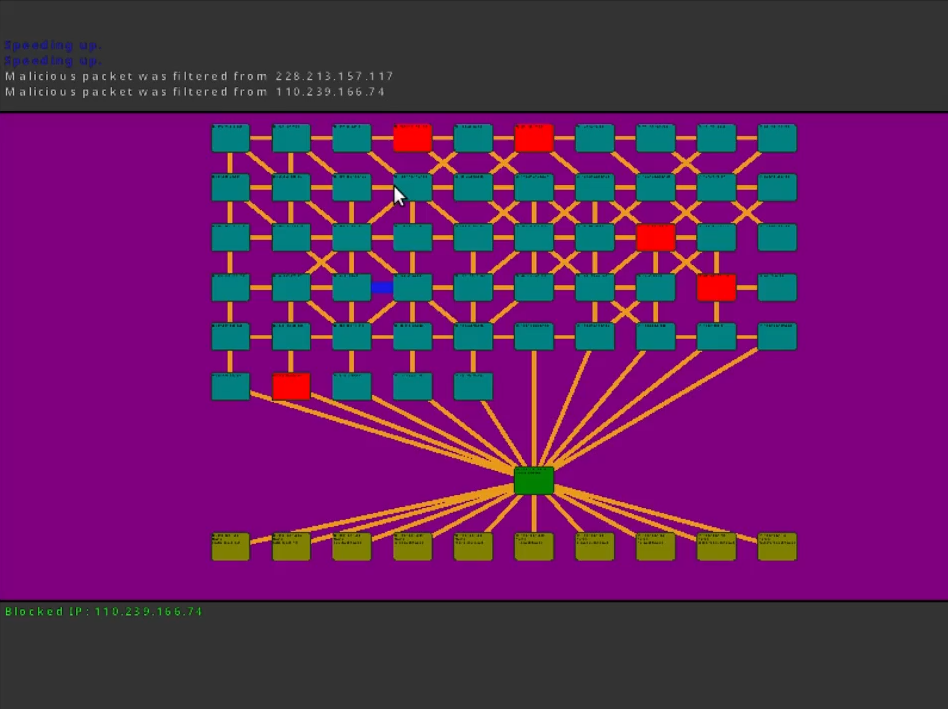
\includegraphics[scale=0.20]{screenshot3.png}

\textit{The simulation is now blocking all packets from the IP address 110.239.166.74, which is a malicious access.}

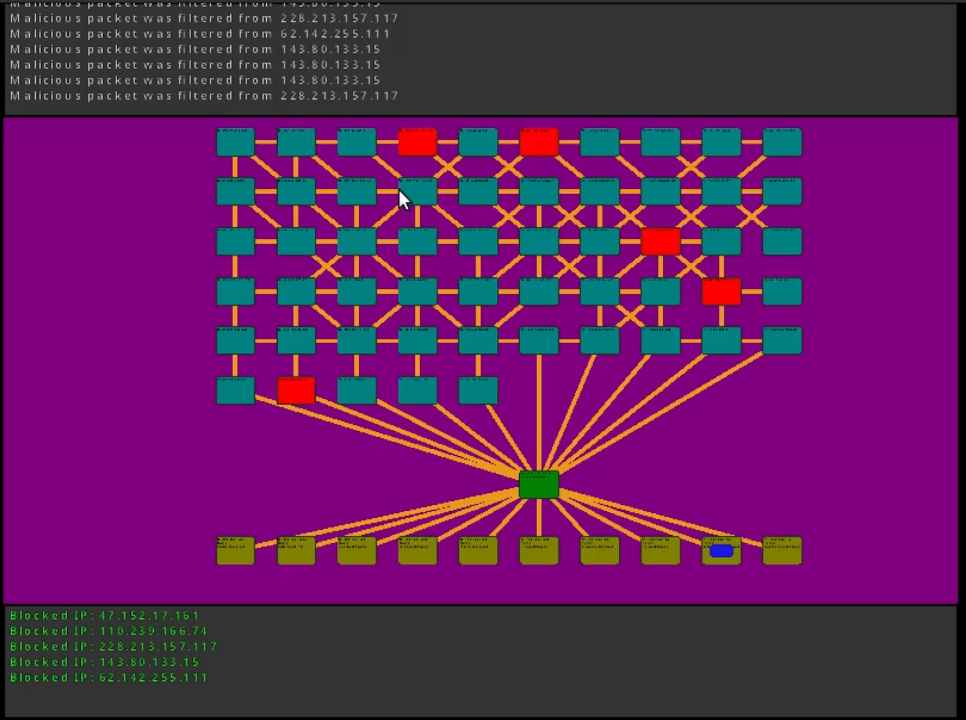
\includegraphics[scale=0.20]{screenshot5.png}

\textit{The simulation has now built up a significant blocklist. However, packets from non-malicious sources (the blue packet at the bottom) are still able to get through.}

In addition, the hosts can change status. On the real internet, the malicious hosts will be taken down, get put up or take over zombie servers. Once every thousand ticks, a malicious server will become benign or a benign server will become malicious. This is to simulate the changing nature of the internet. In addition, to simulate spoofing, sometime malicious flags will also report the wrong IP address.

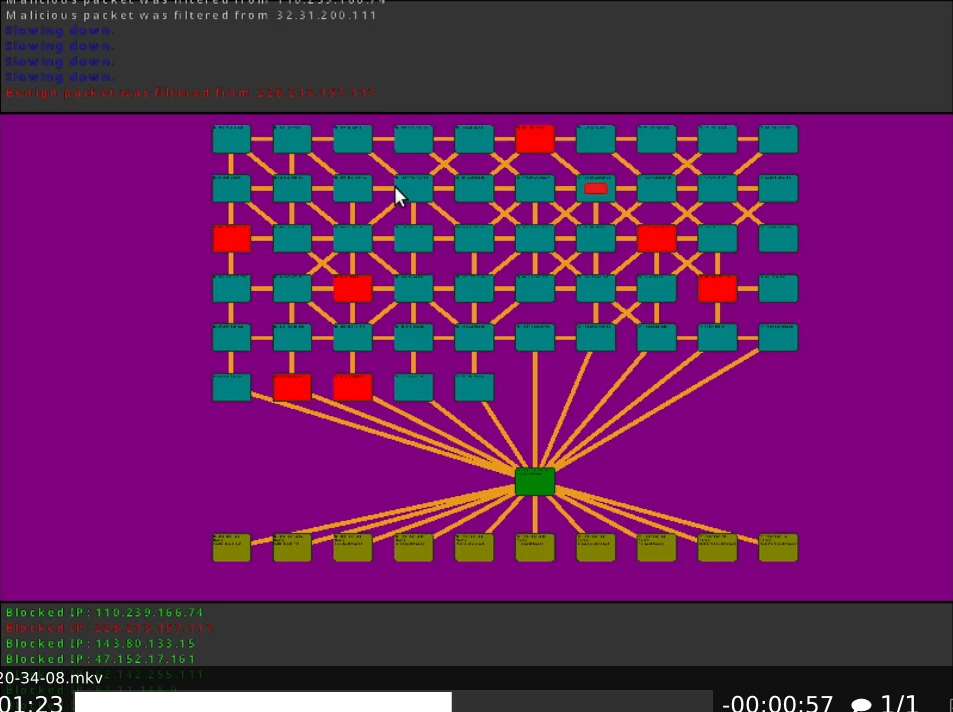
\includegraphics[scale=0.20]{screenshot6.png}

\textit{After some time, the landscape of the network has changed. Some benign machines are now malicious to represent machines being taken over by malicious actors. On the other hand, some malicious machines are now benign to represent malicious actors being taken off of the network. The system is able to detect which actors are now benign and take them off of the list, while realizing which actors are now malicious and adding them to the list.}

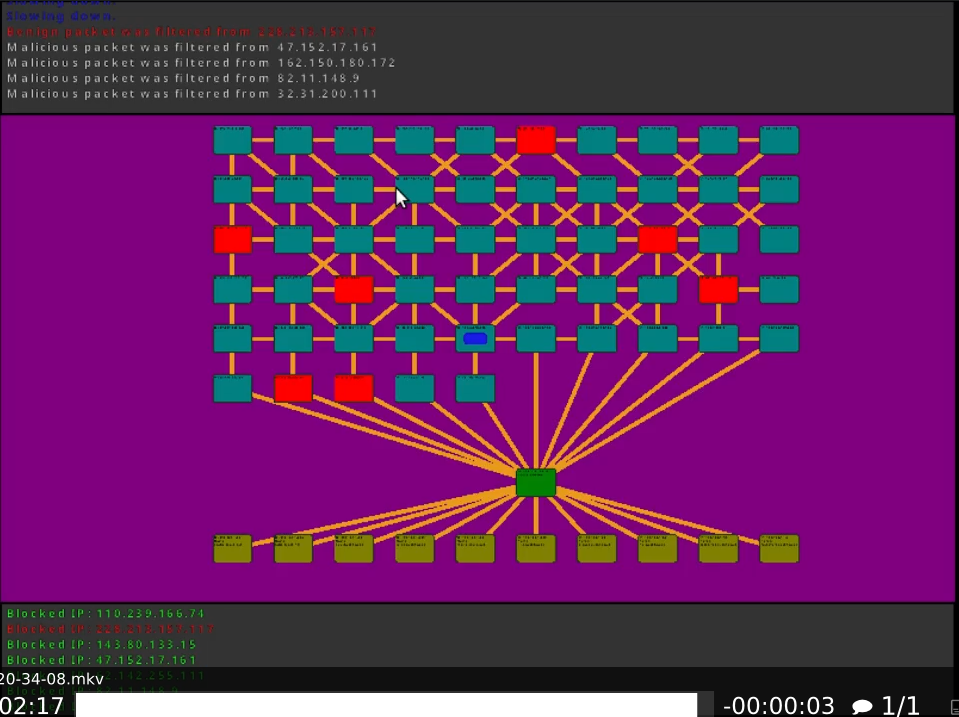
\includegraphics[scale=0.20]{screenshot7.png}

\textit{The system at the end of the simulation. The system has built up a relatively accurate blocklist and is now blocking most malicious packets coming in before they reach their destinations.}

The simulation was run for several dozen million ticks. Although the first million ticks or so had a few malicious packets get through, the simulation was able to block almost all of the malicious traffic. Benign hosts were flagged briefly, but were never blocked for more than a thousand ticks. The simulation was able to block almost all of the malicious traffic, while only blocking benign traffic for a short period of time.

A visualization of this process can be found \href{https://youtu.be/-2nSqtbwnJU}{here}. The source code for the visualization can be found \href{https://github.com/notgull/cs-645-final-project}{here}.

\textbf{4). Existing research}

There are already existing strategies for combining an IDS with a firewall to create an IPS. F rinstance, with the Suricata IDS, there is a supported "nfqueue" mode. This works by installing an agent on the target servers that send packets to Suricata, which decides whether or not they should be sent back. Suricata then sets an Iptables rule that prevents further packets from coming in. However, this still requires setting Suricata in a dedicated "IPS" mode, which avoid the IDS entirely (Digital Ocean, 2021).

\textbf{5). Open Research Challenges/Solution}

The main issue with this method is that is sometimes remembers malicious clients for too long.

Another issue is that it takes some time for it to recognize new clients. This is because the algorithm is based on the assumption that the IDS will flag the same signature multiple times. However, if the IDS has never seen the signature before, it will not flag it. In order to address this issue, the algorithm could be modified to use a different heuristic. For instance, certain rules could decrement the score by a larger amount, or the score could be decremented by a larger amount if the signature is flagged multiple times in a row. This would allow the algorithm to recognize new clients more quickly.

The final issue is the decay rate of the table. The table is currently decayed randomly, with a fixed probability. However, this could be improved by using a more intelligent decay rate. For instance, the table could be decayed based on the number of times a signature is flagged. This would allow the algorithm to adapt to changing conditions, such as new malicious clients and spoofed attacks.

\textbf{6). Conclusions}

While this algorithm is not perfect, it was able to effectively translate the warnings from an IDS into Iptables rules. This is a significant step towards creating a more effective IPS based on IDS technology. The algorithm effectively blocks malicious traffic, while only blocking benign traffic for a short period of time. In addition, it is able to adapt to changing conditions, such as new malicious clients and spoofed attacks.

For the time being, it is recommended to use a dedicated IPS. However, if this algorithm is improved in the futue, it could be used to replace an IPS with an appropriately configured IDS.

\end{multicols}

\newpage

\begin{center}
External Links
\end{center}

Link to the visual demonstration of the simulation: \href{https://youtu.be/-2nSqtbwnJU}{https://youtu.be/-2nSqtbwnJU}

Link to the repository containing the source code: \href{https://github.com/notgull/cs-645-final-project}{https://github.com/notgull/cs-645-final-project}

\newpage

%%%%Works cited
\begin{workscited}

\bibent
Digital Ocean. (2021, Dec 9). \textit{How To Configure Suricata as an Intrusion Prevention System (IPS) on Ubuntu 20.04}. \href{https://www.digitalocean.com/community/tutorials/how-to-configure-suricata-as-an-intrusion-prevention-system-ips-on-ubuntu-20-04}{https://www.digitalocean.com/community/tutorials/how-to-configure-suricata-as-an-intrusion-prevention-system-ips-on-ubuntu-20-04}

\bibent
Mohanakrishnan, R. (2022, Feb 11). \textit{What Is Intrusion Detection and Prevention System?}. Spiceworks. \href{https://www.spiceworks.com/it-security/vulnerability-management/articles/what-is-idps/}{https://www.spiceworks.com/it-security/vulnerability-management/articles/what-is-idps/}

\bibent
NIST. (2015, March 21). \textit{intrusion - Glossary}. \href{https://csrc.nist.gov/glossary/term/intrusion}{https://csrc.nist.gov/glossary/term/intrusion}

\bibent
Patel, A., Qassim, Q. \& Wills, C. (2010), "A survey of intrusion detection and prevention systems", Information Management \& Computer Security, Vol. 18 No. 4, pp. 277-290. https://doi.org/10.1108/09685221011079199 

\bibent
RSI Security. (2021, Sept 20). \textit{How to Implement an Intrusion Prevention System} \href{https://blog.rsisecurity.com/how-to-implement-an-intrusion-prevention-system/}{https://www.emerald.com/insight/content/doi/10.1108/09685221011079199/full/html}

\bibent
Scarfone, K., \& Mell, P. (2007, Feb 20). \textit{Guide to Intrusion Detection and
Prevention Systems (IDPS)}. NIST. \href{https://nvlpubs.nist.gov/nistpubs/legacy/sp/nistspecialpublication800-94.pdf}{https://nvlpubs.nist.gov/nistpubs/legacy/sp/nistspecialpublication800-94.pdf}

\bibent
Software Testing Help. (2023, March 28). \textit{Top 10 BEST Intrusion Detection Systems (IDS)}. \href{https://www.softwaretestinghelp.com/intrusion-detection-systems/}{https://www.softwaretestinghelp.com/intrusion-detection-systems/}

%\bibent
%Allen, R.L. \textit{The American Farm Book; or Compend of Ameri can Agriculture; Being a Practical Treatise on Soils, Manures, Draining, Irrigation, Grasses, Grain, Roots, Fruits, Cotton, Tobacco, Sugar Cane, Rice, and Every Staple Product of the United States with the Best Methods of Planting, Cultivating, and Prep aration for Market.} New York: Saxton, 1849. Print.

%\bibent
%Baker, Gladys L., Wayne D. Rasmussen, Vivian Wiser, and Jane M. Porter. \textit{Century of Service: The First 100 Years of the United States Department of Agriculture.}[Federal Government], 1996. Print.

%\bibent
%Danhof, Clarence H. \textit{Change in Agriculture: The Northern United States, 1820-1870.} Cambridge: Harvard UP, 1969. Print.


\end{workscited}

\end{flushleft}
\end{document}
\}